\documentclass{article}
\usepackage{enumerate}
\usepackage{amsmath}
\usepackage{amssymb}
\usepackage{graphicx}
\usepackage{subfigure}
\usepackage{geometry}
\usepackage{caption}
\usepackage{tikz}
\usepackage{multirow}
\usepackage{array}
\setlength{\parindent}{0pt}


\usepackage{algorithm}
\usepackage{algorithmicx}
\usepackage{algpseudocode}
\renewcommand{\algorithmicrequire}{\textbf{Input:}}
\renewcommand{\algorithmicensure}{\textbf{Output:}}

\geometry{left=3.0cm,right=3.0cm,top=3.0cm,bottom=4.0cm}
\renewcommand{\thesection}{Exercise 10.\arabic{section}}
\title{VE203 Assignment 10}
\author{Liu Yihao 515370910207}
\date{}
\begin{document}
\maketitle

\section{}
\begin{enumerate}[i)]
\item
Since there isn't a circuit with three vertices, and $e=14$, $v=8$, $e>2v-4$, so it is not a planner graph.
\item \ 
\begin{center}
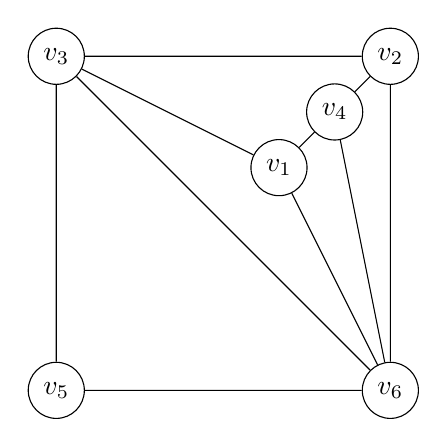
\begin{tikzpicture}[scale=2, bend angle=22.5]
\tikzstyle{every node}=[draw,shape=circle];
\path (45:1.5cm) node (v2) {$v_2$};
\path (135:1.5cm) node (v3) {$v_3$};
\path (225:1.5cm) node (v5) {$v_5$};
\path (315:1.5cm) node (v6) {$v_6$};
\path (45:0.5cm) node (v1) {$v_1$};
\path (45:1cm) node (v4) {$v_4$};
\draw
(v2) -- (v3) -- (v5) -- (v6) -- (v2)
(v2) -- (v4) -- (v6) -- (v1) -- (v3) -- (v6)
(v1) -- (v4)
;
\end{tikzpicture}
\end{center}
\item
Since $e=18$, $v=7$, $e>3v-6$, so it is not a planner graph.
\end{enumerate}

\section{}
Since it is a full $m$-$ary$ balanced tree of height $h$, it must contain a perfect 
$m$-$ary$ tree of height $h-1$, which has $m^{h-1}$ leaves. If there are $km,k\in[1,m]\cap N$ leaves of height $h$, then there are $m^{h-1}+k(m-1)$ leaves, which is more than $m^{h-1}$ leaves.\\
Since $l\in[m^{h-1}+(m-1),m^h]$, and a full $m$-$ary$ balanced tree of height $h-1$
has at most $m^{h-1}$ leaves, a full $m$-$ary$ balanced tree of height $h+1$
has at least $m^h+(m-1)$ leaves, $h=[\log_ml]$.

\section{}
\begin{algorithm}
\begin{algorithmic}[1]
	\Require Four coins with weight $m_1,m_2,m_3,m_4$ (unknown), one of them may be counterfeit
	\Ensure The counterfeit coin and whether it is heavier or lighter (if exists)
	\State Compare $m_1$ and $m_2$
	\State Compare $m_3$ and $m_4$
	\If{$m_1\neq m_2$}
		\State Compare $min(m_1,m_2)$ and $m_3$
		\If{$min(m_1,m_2)=m_3$}
			\State $max(m_1,m_2)$ is counterfeit (heavier)
		\Else
			\State $min(m_1,m_2)$ is counterfeit (lighter)
		\EndIf
	\ElsIf{$m_3\neq m_4$}
		\State Compare $min(m_3,m_4)$ and $m_1$
		\If{$min(m_3,m_4)=m_1$}
			\State $max(m_3,m_4)$ is counterfeit (heavier)
		\Else
			\State $min(m_3,m_4)$ is counterfeit (lighter)
		\EndIf
	\Else
		\State No coin is counterfeit
	\EndIf
\end{algorithmic}
\end{algorithm}

At most three weighings are needed.

\newpage


\section{}
If there is n symbols $a_1,...,a_n$ with frequencies $p_1,...,p_n$, whose bits are $b_1,...,b_n$. If $p_1>...>p_n$ and $b_1<...<b_n$, according to sequence inequality, we can obtain that 
$$\sum_{i=1}^np_ib_i\leqslant\sum_{i=1,j=f(i)}^np_ib_j$$
where $i,j\in[1,n]\cap N$ and $f(i)$ is a random bijective function from $i$ to $j$
Since the Huffman codes use the fewest bits for the biggest frequency, which satisfy the model above, it uses the fewest bits in total.

\section{}
\begin{enumerate}[i)]
\item \ 
\begin{center}
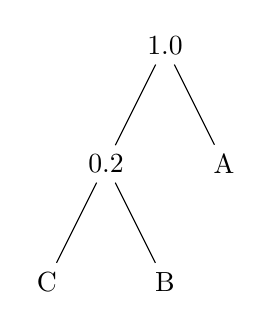
\begin{tikzpicture}[scale=1]
\node {1.0}
	child {
		node {0.2}
		child { node {C} }
		child { node {B} }
	}
	child { node {A} };
\end{tikzpicture}
\end{center}
$$C:00,\quad B:01,\quad A:1$$
\item
$$AA:0.64,\quad AB:0.152,\quad AC:0.008$$
$$BA:0.152,\quad BB:0.0361,\quad BC:0.0019$$
$$CA:0.008,\quad CB:0.0019,\quad CC:0.0001$$
\begin{center}
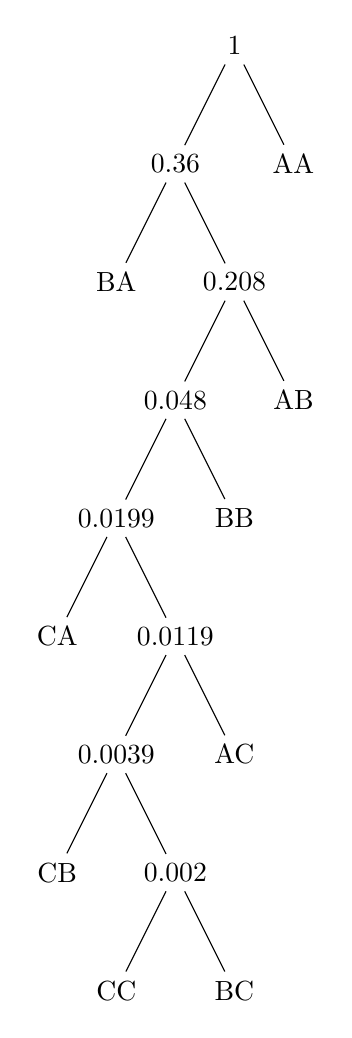
\begin{tikzpicture}[scale=1]
\node {1}
child { node{0.36}
	child { node {BA} }
	child { node{0.208}
		child { node{0.048}
			child { node{0.0199}
				child { node {CA} }
				child { node{0.0119}
					child { node {0.0039}
						child { node {CB} }
						child { node {0.002}
							child { node {CC} }
							child { node {BC} }
						}			
					}
					child { node {AC} }
				}
			}
			child { node {BB} }
		}
		child { node {AB} }
	}
}
child { node{AA} };
\end{tikzpicture}
\end{center}
$$AA:1,\quad AB:011,\quad AC:010011$$
$$BA:00,\quad BB:0101,\quad BC:01001011$$
$$CA:01000,\quad CB:0100100,\quad CC:01001010$$
\item
In part i),
$$\overline{N}=1\times0.8+2\times0.19+2\times0.01=1.2$$
In part ii),
$$\overline{N}=\frac{1}{2}\Big[1\times0.64+(2+3)\times0.152+4\times0.0361
+(5+6)\times0.008+(7+8\times0.0019)+8\times0.0001\Big]=0.8489$$
So part ii) is more efficient.
\end{enumerate}

\section{}
\begin{enumerate}[i)]
\item \

\begin{minipage}{0.48\linewidth}
Step 1:
\begin{center}
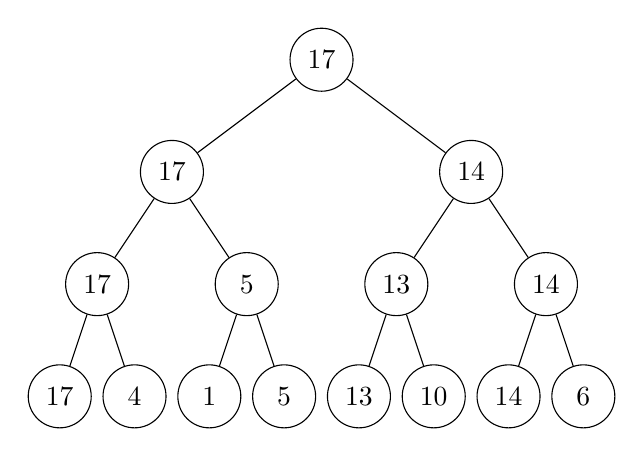
\begin{tikzpicture}[scale=0.95]
\tikzstyle{every node}=[draw,shape=circle,minimum size=0.8cm];
\node {17}[sibling distance=4cm]
child { node {17}[sibling distance=2cm]
	child {
		node {17}[sibling distance=1cm]
		child { node {17} }
		child { node {4} }
	}
	child {
		node {5}[sibling distance=1cm]
		child { node {1} }
		child { node {5} }
	}
}
child { node {14}[sibling distance=2cm]
	child {
		node {13}[sibling distance=1cm]
		child { node {13} }
		child { node {10} }
	}
	child {
		node {14}[sibling distance=1cm]
		child { node {14} }
		child { node {6} }
	}
};
\end{tikzpicture}
\end{center}
\end{minipage}
\hfill
\begin{minipage}{0.48\linewidth}
Step 2:
\begin{center}
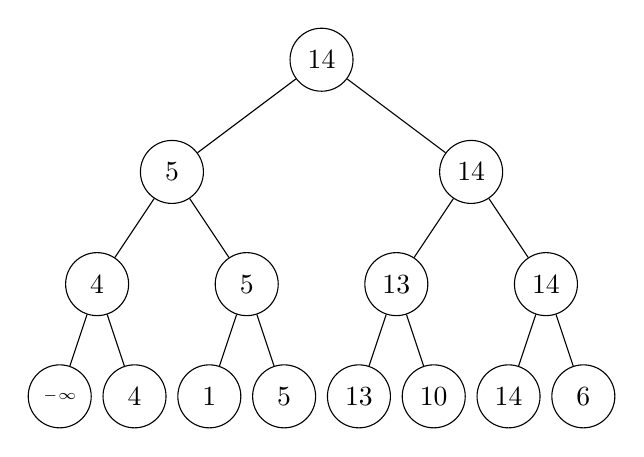
\begin{tikzpicture}[scale=0.95]
\tikzstyle{every node}=[draw,shape=circle,minimum size=0.8cm];
\node {14}[sibling distance=4cm]
child { node {5}[sibling distance=2cm]
	child {
		node {4}[sibling distance=1cm]
		child { node {\tiny{$-\infty$}} }
		child { node {4} }
	}
	child {
		node {5}[sibling distance=1cm]
		child { node {1} }
		child { node {5} }
	}
}
child { node {14}[sibling distance=2cm]
	child {
		node {13}[sibling distance=1cm]
		child { node {13} }
		child { node {10} }
	}
	child {
		node {14}[sibling distance=1cm]
		child { node {14} }
		child { node {6} }
	}
};
\end{tikzpicture}
\end{center}
\end{minipage}
\vfill
\begin{minipage}{0.48\linewidth}
Step 3:
\begin{center}
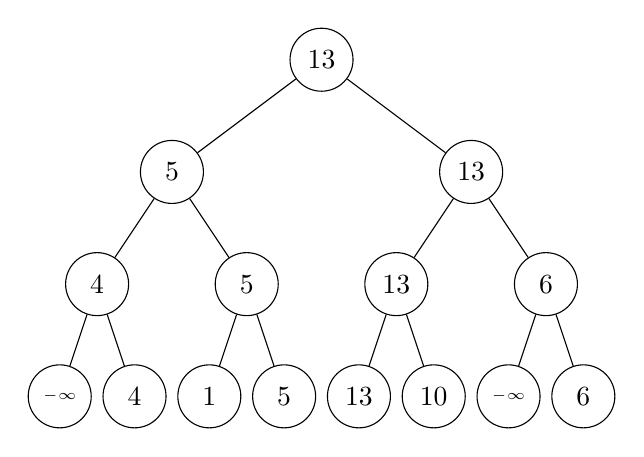
\begin{tikzpicture}[scale=0.95]
\tikzstyle{every node}=[draw,shape=circle,minimum size=0.8cm];
\node {13}[sibling distance=4cm]
child { node {5}[sibling distance=2cm]
	child {
		node {4}[sibling distance=1cm]
		child { node {\tiny{$-\infty$}} }
		child { node {4} }
	}
	child {
		node {5}[sibling distance=1cm]
		child { node {1} }
		child { node {5} }
	}
}
child { node {13}[sibling distance=2cm]
	child {
		node {13}[sibling distance=1cm]
		child { node {13} }
		child { node {10} }
	}
	child {
		node {6}[sibling distance=1cm]
		child { node {\tiny{$-\infty$}} }
		child { node {6} }
	}
};
\end{tikzpicture}
\end{center}
\end{minipage}
\hfill
\begin{minipage}{0.48\linewidth}
Step 4:
\begin{center}
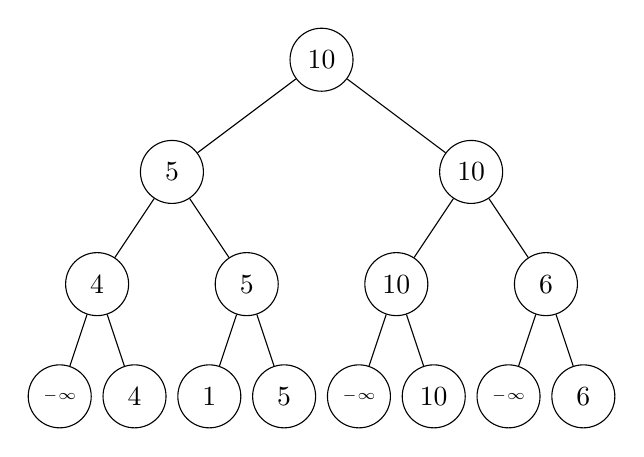
\begin{tikzpicture}[scale=0.95]
\tikzstyle{every node}=[draw,shape=circle,minimum size=0.8cm];
\node {10}[sibling distance=4cm]
child { node {5}[sibling distance=2cm]
	child {
		node {4}[sibling distance=1cm]
		child { node {\tiny{$-\infty$}} }
		child { node {4} }
	}
	child {
		node {5}[sibling distance=1cm]
		child { node {1} }
		child { node {5} }
	}
}
child { node {10}[sibling distance=2cm]
	child {
		node {10}[sibling distance=1cm]
		child { node {\tiny{$-\infty$}} }
		child { node {10} }
	}
	child {
		node {6}[sibling distance=1cm]
		child { node {\tiny{$-\infty$}} }
		child { node {6} }
	}
};
\end{tikzpicture}
\end{center}
\end{minipage}
\vfill
\begin{minipage}{0.48\linewidth}
Step 5:
\begin{center}
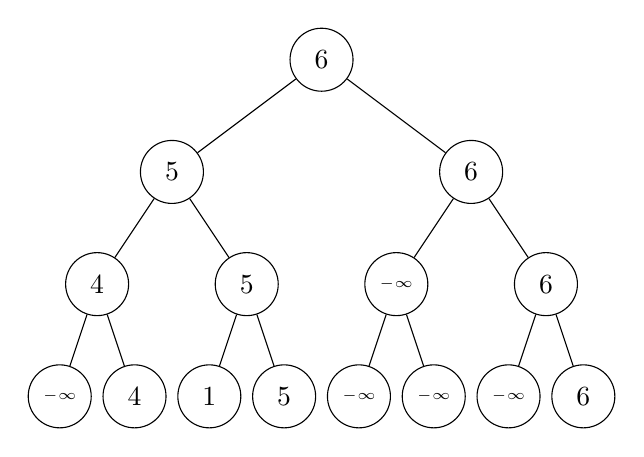
\begin{tikzpicture}[scale=0.95]
\tikzstyle{every node}=[draw,shape=circle,minimum size=0.8cm];
\node {6}[sibling distance=4cm]
child { node {5}[sibling distance=2cm]
	child {
		node {4}[sibling distance=1cm]
		child { node {\tiny{$-\infty$}} }
		child { node {4} }
	}
	child {
		node {5}[sibling distance=1cm]
		child { node {1} }
		child { node {5} }
	}
}
child { node {6}[sibling distance=2cm]
	child {
		node {\tiny{$-\infty$}}[sibling distance=1cm]
		child { node {\tiny{$-\infty$}} }
		child { node {\tiny{$-\infty$}} }
	}
	child {
		node {6}[sibling distance=1cm]
		child { node {\tiny{$-\infty$}} }
		child { node {6} }
	}
};
\end{tikzpicture}
\end{center}
\end{minipage}
\hfill
\begin{minipage}{0.48\linewidth}
Step 6:
\begin{center}
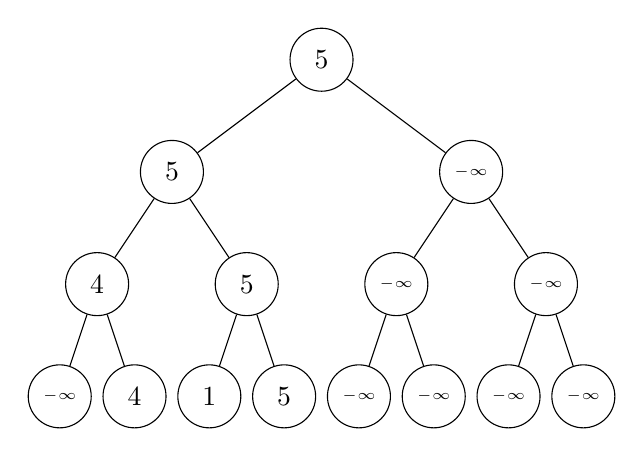
\begin{tikzpicture}[scale=0.95]
\tikzstyle{every node}=[draw,shape=circle,minimum size=0.8cm];
\node {5}[sibling distance=4cm]
child { node {5}[sibling distance=2cm]
	child {
		node {4}[sibling distance=1cm]
		child { node {\tiny{$-\infty$}} }
		child { node {4} }
	}
	child {
		node {5}[sibling distance=1cm]
		child { node {1} }
		child { node {5} }
	}
}
child { node {\tiny{$-\infty$}}[sibling distance=2cm]
	child {
		node {\tiny{$-\infty$}}[sibling distance=1cm]
		child { node {\tiny{$-\infty$}} }
		child { node {\tiny{$-\infty$}} }
	}
	child {
		node {\tiny{$-\infty$}}[sibling distance=1cm]
		child { node {\tiny{$-\infty$}} }
		child { node {\tiny{$-\infty$}} }
	}
};
\end{tikzpicture}
\end{center}
\end{minipage}
\vfill
\begin{minipage}{0.48\linewidth}
Step 7:
\begin{center}
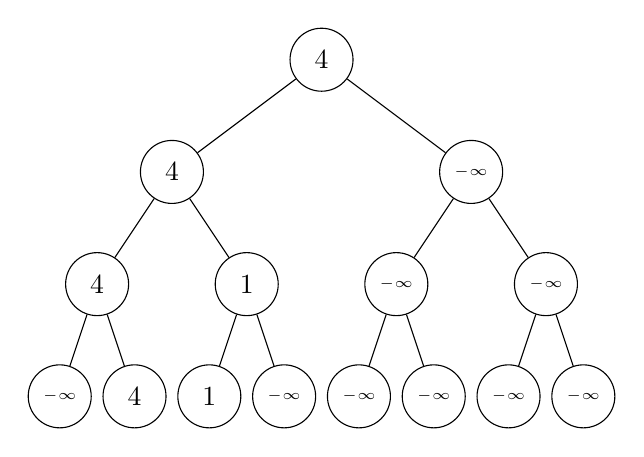
\begin{tikzpicture}[scale=0.95]
\tikzstyle{every node}=[draw,shape=circle,minimum size=0.8cm];
\node {4}[sibling distance=4cm]
child { node {4}[sibling distance=2cm]
	child {
		node {4}[sibling distance=1cm]
		child { node {\tiny{$-\infty$}} }
		child { node {4} }
	}
	child {
		node {1}[sibling distance=1cm]
		child { node {1} }
		child { node {\tiny{$-\infty$}} }
	}
}
child { node {\tiny{$-\infty$}}[sibling distance=2cm]
	child {
		node {\tiny{$-\infty$}}[sibling distance=1cm]
		child { node {\tiny{$-\infty$}} }
		child { node {\tiny{$-\infty$}} }
	}
	child {
		node {\tiny{$-\infty$}}[sibling distance=1cm]
		child { node {\tiny{$-\infty$}} }
		child { node {\tiny{$-\infty$}} }
	}
};
\end{tikzpicture}
\end{center}
\end{minipage}
\hfill
\begin{minipage}{0.48\linewidth}
Step 8:
\begin{center}
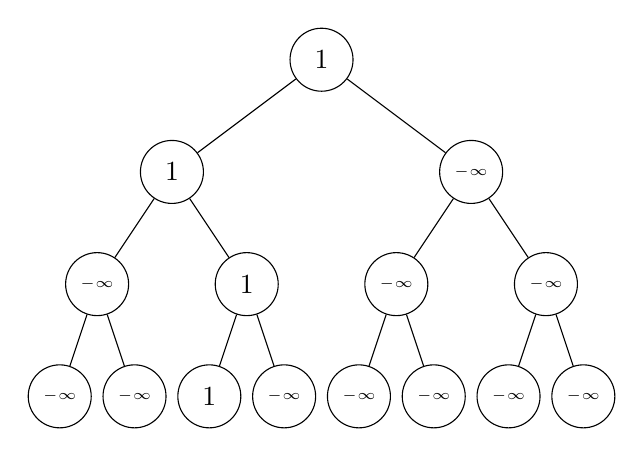
\begin{tikzpicture}[scale=0.95]
\tikzstyle{every node}=[draw,shape=circle,minimum size=0.8cm];
\node {1}[sibling distance=4cm]
child { node {1}[sibling distance=2cm]
	child {
		node {\tiny{$-\infty$}}[sibling distance=1cm]
		child { node {\tiny{$-\infty$}} }
		child { node {\tiny{$-\infty$}} }
	}
	child {
		node {1}[sibling distance=1cm]
		child { node {1} }
		child { node {\tiny{$-\infty$}} }
	}
}
child { node {\tiny{$-\infty$}}[sibling distance=2cm]
	child {
		node {\tiny{$-\infty$}}[sibling distance=1cm]
		child { node {\tiny{$-\infty$}} }
		child { node {\tiny{$-\infty$}} }
	}
	child {
		node {\tiny{$-\infty$}}[sibling distance=1cm]
		child { node {\tiny{$-\infty$}} }
		child { node {\tiny{$-\infty$}} }
	}
};
\end{tikzpicture}
\end{center}
\end{minipage}
\item
$$C=\sum_{i=0}^{k-1}2^{i}=2^k-1=n-1$$
\item
When searching downwards, there are $\log_2n$ comparisons to find the larger node.\\
When backtracking, there are $\log_2n$ comparisons to update the node.\\
So there are $2\log_2n$ comparisons in total.
\item
$$O(n-1+2(n-1)\log_2n)=O(n\log n)$$
\end{enumerate}


\end{document}
